% =============================================================================
% sections/design/rover/electronics_overview.tex  -  Electronics Overview
% Teams: electronics (best guess - unconfirmed) / Status: EXAMPLE (scope approximation)
%
% EXAMPLE CONTENT for scope/layout approximation - not final report text.
% Adapted from the Preliminary Report's "Battery Configuration and
% Hot-Swap Design" / "Power Distribution and Regulation" subsections,
% trimmed to minimal prose. Marked with \exampleflag on its heading in the
% assembler.
%
% Image is a placeholder (teams/electronics/figures/power_distribution_schematic.png)
% - swap it for the real schematic by overwriting the same file.
% =============================================================================

The rover's power system is built around a \qty{48}{\volt} DC bus, with
three to four hot-swappable commercial lithium-ion battery modules
(\qty{48}{\volt}, \qty{12}{\ampere\hour} each) connected in parallel,
giving \qtyrange{36}{48}{\ampere\hour} of capacity depending on mission
demand. Modules mount on a rail-based hot-swap dock for tool-free
replacement in the field and include integrated BMS protection with
current sharing across modules. Power is split into two segments, shown in
\autoref{fig:power_distribution_schematic}: an always-on Safety and
Control Segment, powered directly off the bus ahead of the main
contactor, that regulates \qty{24}{\volt}, \qty{5}{\volt}, and
\qty{3.3}{\volt} rails for the emergency-stop system, control logic, and
communications even with main power disconnected; and a Main Power
Segment, activated via the main contactor, that distributes
\qty{48}{\volt}, \qty{24}{\volt}, \qty{5}{\volt}, and \qty{3.3}{\volt}
rails to all operational consumers.

\begin{figure}[!htbp]
    \centering
    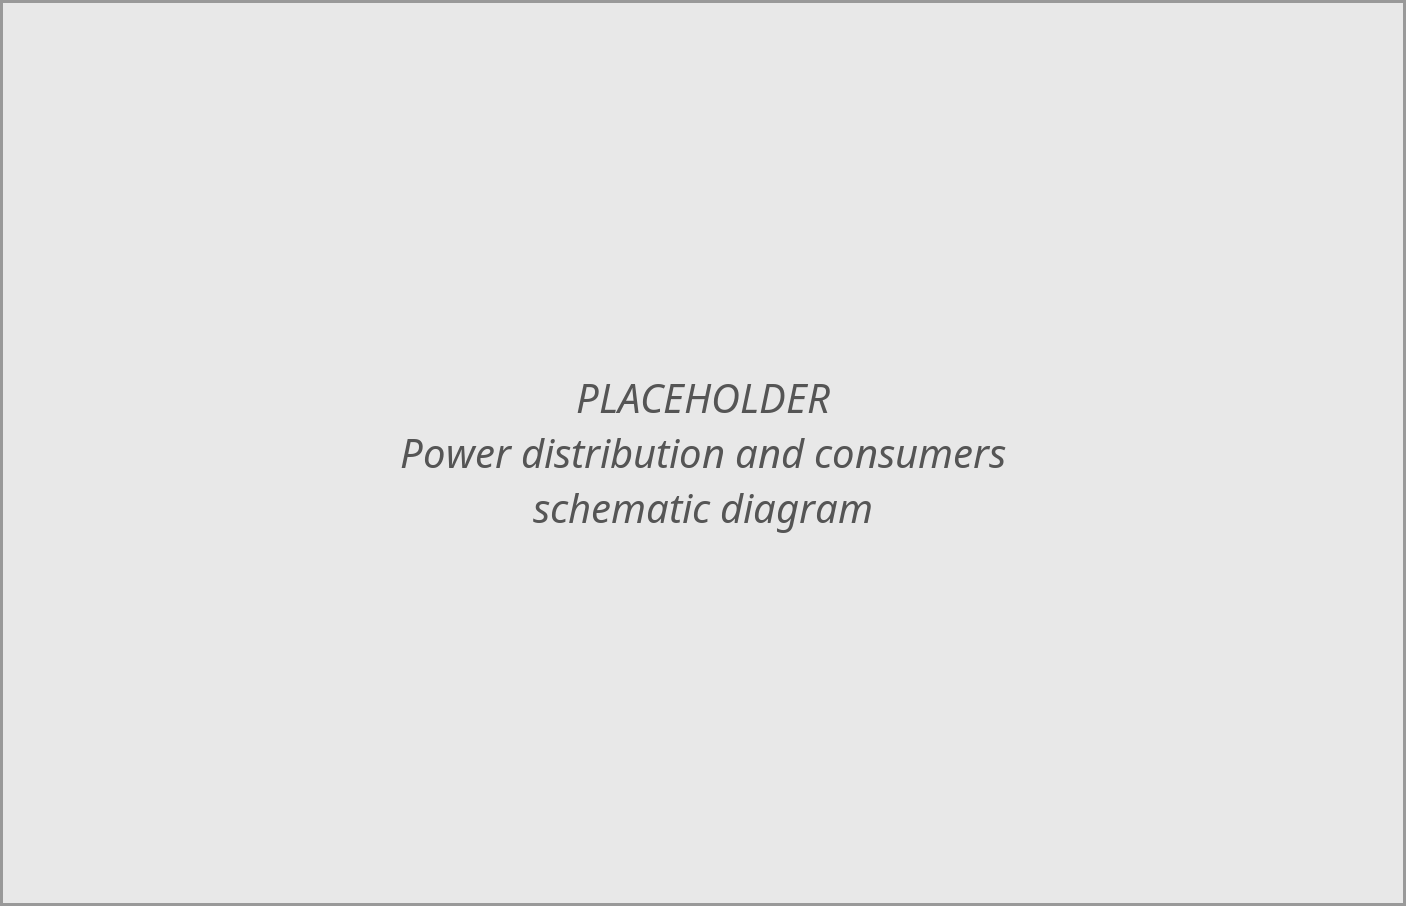
\includegraphics[width=0.85\linewidth]{teams/electronics/figures/power_distribution_schematic}
    \caption{Power distribution and consumers schematic diagram}
    \label{fig:power_distribution_schematic}
\end{figure}
